\section{Desarrollo de software}

\subsection{Elección de arquitectura}
La decisión de software a usar depende del controlador a usar, poder de cálculo disponible on board, interfazes de perifericos y funcionalidad deseada.

El controlador a usar es el ARM Cortex-A72 que sería comprado en el paquete comercial conocido como \textit{Raspberry Pi 4B+}. El producto provee salidas para los siguientes usos

\begin{itemize}
    \item UART
    \item SPI
    \item I$^2$C
    \item GPIO
\end{itemize}

La Raspberry Pi provee un entorno con linux instalado que permite la programación con virtualmente cualquier lenguaje de programación en existencia. Dado estas condiciones, el lenguaje de programación elegido es \textbf{Go} (Golang) debido a los siguientes puntos

\begin{itemize}
    \item Seguro - Modelo de memoria Go, sistema de tipado fuerte
    \item Simple - Claridad de sintaxis
    \item Concurrencia - Crear corutinas es simple, paralelizar corutinas es trivial
    \item Rendimiento - Superior a Python, Java y Matlab. Comparable a C
    \item Estable - \textit{The Go 1 promise} (La promesa Go 1)
    \item Comprobado -  Usado en sistemas de alto-riesgo/alta-complejidad (Kubernetes, Docker, Go-HEP)
\end{itemize}
\clearpage
\subsection{Flujo de control}
\begin{figure}[!htb]
    \centering
    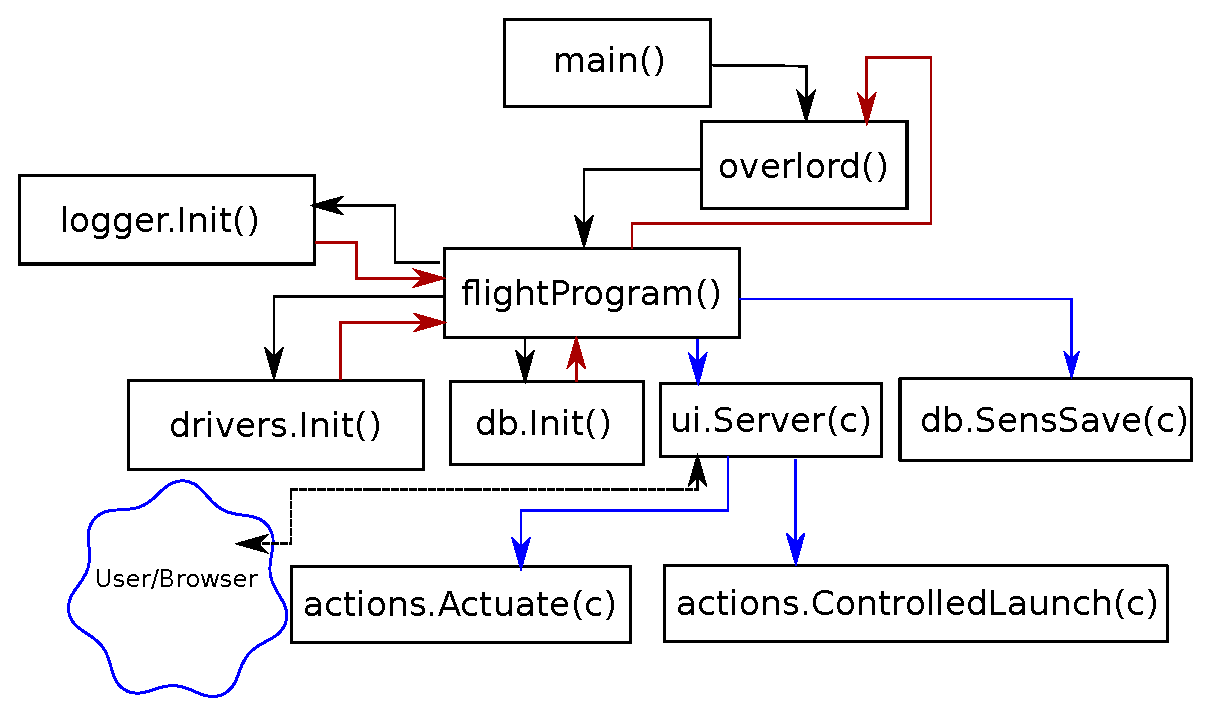
\includegraphics[width=0.7\textwidth]{fig/cfg_flightprogram.eps}
    \caption{Gráfico de flujo de control (CFG) del programa de vuelo. Las lineas de flujo azules son corutinas independientes al programa principal. Las lineas negras son flujo del programa principal. Las lineas rojas son flujo del programa principal al encontrar un error.}
    \label{fig:flightProgram}
\end{figure}

Se ilustra el flujo de control a grandes rasgos usando un CFG en la figura \ref{fig:flightProgram}. El programa principal corre la rutina \texttt{overlord} que a su vez comanda \texttt{flightProgram} y espera que esta devuelva control a \texttt{overlord}. El proposito de \texttt{overlord} es guardar el estado del vehículo y ante una falla irrecuperable en \texttt{flightProgram}, terminar con todas las corutinas generadas por \texttt{flightProgram} y sus afiliadas y a su vez reiniciar \texttt{flightProgram} nuevamente con el último estado antes de la falla.










